\documentclass[9pt,a4paper]{article}

\usepackage[french]{babel}
\usepackage{graphicx} % Required for inserting images
\usepackage{fancyhdr}
\usepackage{fancyvrb}
\usepackage[a4paper,top=2cm,bottom=2cm,left=3cm,right=3cm,marginparwidth=1.75cm]{geometry}
\usepackage{amssymb} % ensemble des réels, etc
\usepackage{amsmath}
\usepackage{stmaryrd} % pour utiliser les intervalles d'entiers
\usepackage{enumitem} % pour utiliser les points dans les listes
\usepackage{pst-all}
\usepackage{tcolorbox}

\newtheorem{rem}{Remarque}

\usepackage[linesnumbered, ruled, vlined]{algorithm2e}
\renewcommand{\algorithmcfname}{Algorithme}
\SetKwInput{KwData}{Données}
\SetKwInput{KwRes}{Résultat}
\SetKwProg{Fonction}{Fonction}{}{FinFonction}
\SetKwIF{Si}{SinonSi}{Sinon}{Si}{alors}{SinonSi}{Sinon}{FinSi}
\SetKwFor{Pour}{Pour}{faire}{FinPour}
\SetKwFor{Tq}{Tant que}{faire}{FinTantque}
\SetKw{Renvoyer}{Renvoyer}
\usepackage{algpseudocode}

\pagestyle{fancy}
\title{Minimisation d'une fonctionnelle quadratique}
\author{Kelvin LEFORT Selim LIMAM}
\date
\begin{document}

\maketitle
\cfoot{MACS 2 - Sup Galilée - Institut Galilée - Université Sorbonne Paris Nord}
\rfoot{\thepage}
\tableofcontents % écrit la table des matières
\newpage

\section{Introduction}
\subsection{Description du problème}
Soient $A$ une matrice symétrique définie positive de taille $n$ et  $b$ un vecteur de taille $n$. On considère la fonctionnelle quadratique
$$
f(x) = \frac{1}{2}(Ax,x) - (b,x)
$$
On rappelle que $\nabla f(x) = Ax-b$ et $(f''(x)h,h) = (Ah,h)$.\newline
Le problème que nous nous posons est celui de la minimisation de cette fonctionnelle.
\subsection{Existence et unicité du point de minimum}
La première question qu'on se pose face à ce type de problème est celle de l'existence d'une solution et si possible de son unicité.\newline
Pour ce faire, on peut montrer que $f$ est $\alpha$-convexe, pour un certain $\alpha > 0$.\newline
En effet, en appliquant le théorème spectral ($A$ est symétrique), on montre que
$$
(Ah,h) \geqslant \alpha \Vert h \Vert_2^2
$$
avec $\alpha = (\min_{j=1,...,n}\lambda_j)$, où les $\lambda_j$ sont les valeurs propres de $A$ (comptées avec leur multiplicité).\newline
Mais puisque $A$ est en plus définie positive, alors toutes ses valeurs propres sont strictement positives, i.e. $\alpha > 0$.\newline
Remarquons aussi que $f$ est continue en tant que fonctionnelle quadratique.\newline
Ainsi, par le théorème d'existence et d'unicité (en dimension finie ou infinie), $f$ admet un unique point de minimum, qu'on note $x^*$.
\subsection{Caractérisation du point de minimum}
Maintenant qu'on sait que $x^*$ existe et est unique, la prochaine question qu'on se pose dans ce type de problème est comment caractériser cette solution.\newline
La condition d'optimalité du premier ordre nous indique que $\nabla f(x^*) = 0$, autrement dit $Ax^* - b = 0$, c'est-à-dire $x^* = A^{-1}b$ (A est symétrique définie positive, donc inversible).\newline
\begin{tcolorbox}[colback = green!10!white]
    \begin{rem}
    Le point de minimum de $f$ est la solution du système linéaire
    $$
    Ax = b
    $$
    Ainsi, minimiser $f$ est équivalent à résoudre ce système linéaire.
    \end{rem}
\end{tcolorbox}
\subsection{Objectif des algorithmes}
Dans ce cas bien précis (celui d'une fonctionnelle quadratique), l'utilisation des algorithmes n'est pas nécéssaire car on connait la solution. Néanmoins, dans le cas général, on peut savoir que la fonctionnelle admet un point de minimum (et si possible qu'il est unique) grâce à des théorèmes d'existence et d'unicité sans pouvoir le caractériser. C'est ici qu'intervient les algorithmes. Leur but est construire une suite de points qui converge vers un/le point de minimum (local ou global). Ainsi, en allant suffisamment loin dans le calcul des itérés de la suite, on pourra avoir à disposition une "bonne" approximation de la solution.\newline
Nous allons programmer trois de ces algorithmes (ce sera des algorithmes de descente du gradient) et nous pourrons les tester avec $f$ comme fonctionnelle. L'avantage ici est qu'on connait la solution exacte donc on peut effectuer des tests sur ces algorithmes.
\section{Algorithmes}
On prendra $A =
\begin{pmatrix}
    2 & -1\\
    -1 & 2
\end{pmatrix}$, $x^* =
\begin{pmatrix}
    1\\
    2
\end{pmatrix}$ et donc $b = Ax^* = 
\begin{pmatrix}
    0\\
    3
\end{pmatrix}$ pour tester les différents algorithmes.\newline
De plus, on prendra \textit{tolerance} $=$ eps et \textit{itermax} $=$ 1000 (voir les codes pour comprendre leurs significations).
\subsection{Méthode du gradient à pas constant}
\subsubsection{Description de la méthode}
Soient $\rho > 0$ et $x_0 \in \mathbb{R}^n$. La méthode du gradient à pas constant consiste à construire la suite $(x_k)_{k \in \mathbb{N}}$ de la manière suivante
$$
x_{k+1} = x_k - \rho \nabla f(x_k), \forall k \in \mathbb{N}
$$
\subsubsection{Test de la méthode}
Pour tester cette méthode, on a pris $\rho = 0,1$ et $x_0 = 
\begin{pmatrix}
    0\\
    0
\end{pmatrix}$.\newline
On constate alors que l'algorithme converge en $331$ itérérations.\newline
Veuillez trouver ci-dessous une représentation graphique de $f$ ainsi que la suite des itérés $(x_k,f(x_k))$.
\begin{figure}[h]
    \centering
    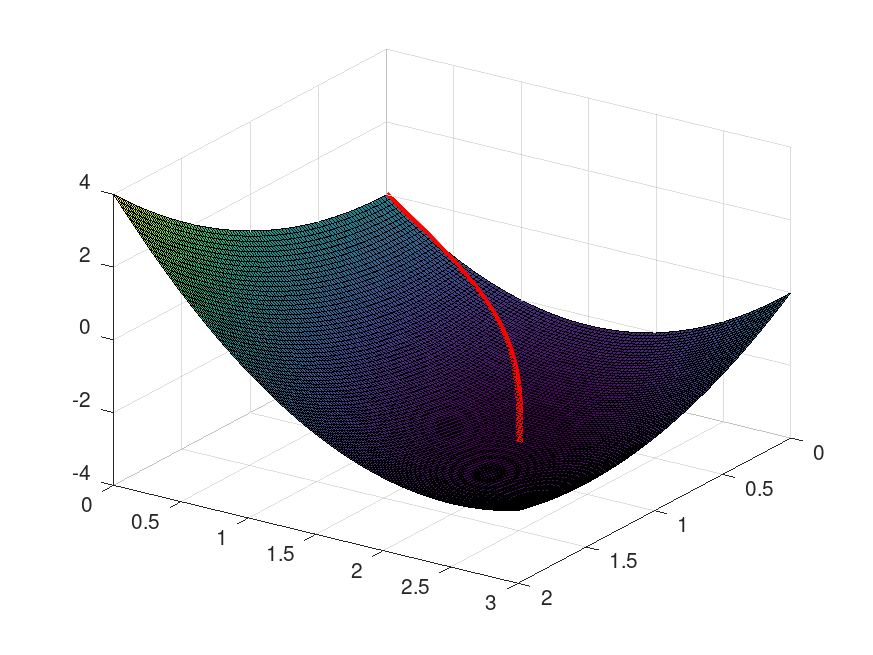
\includegraphics[scale=0.25]{GradientPasConstant.png}
    \caption{Représentation graphique de $f$ et de la suite des itérés $(x_k,f(x_k))$}
    \label{fig:enter-label}
\end{figure}\newline
On observe bien que la suite "descend" vers le minimum de $f$, d'où le nom de ce type d'algorithme.
\subsubsection{Etude de la convergence}
On se demande alors pour quelles valeurs de $\rho$ et $x_0$ cette méthode converge.
\paragraph{Théorique}
Pour tout $k \in \mathbb{N}$, on pose $e_k = x_k - x^*$ et pour tout $M \in \mathcal{M}_n(\mathbb{R})$, $r_{\sigma}(M)$ désigne le rayon spectral de $M$.\newline
On montre alors que pour tout $k \in \mathbb{N}$
$$
e_{k+1} = (I - \rho A)e_k
$$
D'après un résultat d'analyse numérique, la suite $(e_k)_{k \in \mathbb{N}}$ converge vers $0$ si et seulement si $r_{\sigma}(I - \rho A) < 1$. Il suffit donc d'étudier la fonction $\rho \longmapsto r_{\sigma}(I - \rho A)$.\newline
Commençons par calculer les valeurs propres de $I - \rho A$.\newline
La matrice $A$ étant symétrique, il existe une matrice $P$ orthogonale et une matrice $D$ diagonale telles que
$$
D = P^T A P
$$
Donc
$$
I - \rho D = P^T (I - \rho A) P
$$
Ainsi, en notant $\lambda_i$ les valeurs propres de $A$, les valeurs propres de $I - \rho A$ sont données par $1 - \rho \lambda_i$.\newline
Pour les tests, on a pris $A =
\begin{pmatrix}
    2 & -1\\
    -1 & 2
\end{pmatrix}$. Ses valeurs propres sont $1$ et $3$ et donc les valeurs propres de $I - \rho A$ sont $1 - \rho$ et $1 - 3 \rho$. D'où $r_{\sigma}(I - \rho A) = \max\{|1 - \rho|,|1 - 3 \rho|\}$. La fonction $\rho \longmapsto r_{\sigma}(I - \rho A)$ est donc simple à étudier. 
\newpage
Voici sa représentation graphique.
\begin{figure}[h]
    \centering
    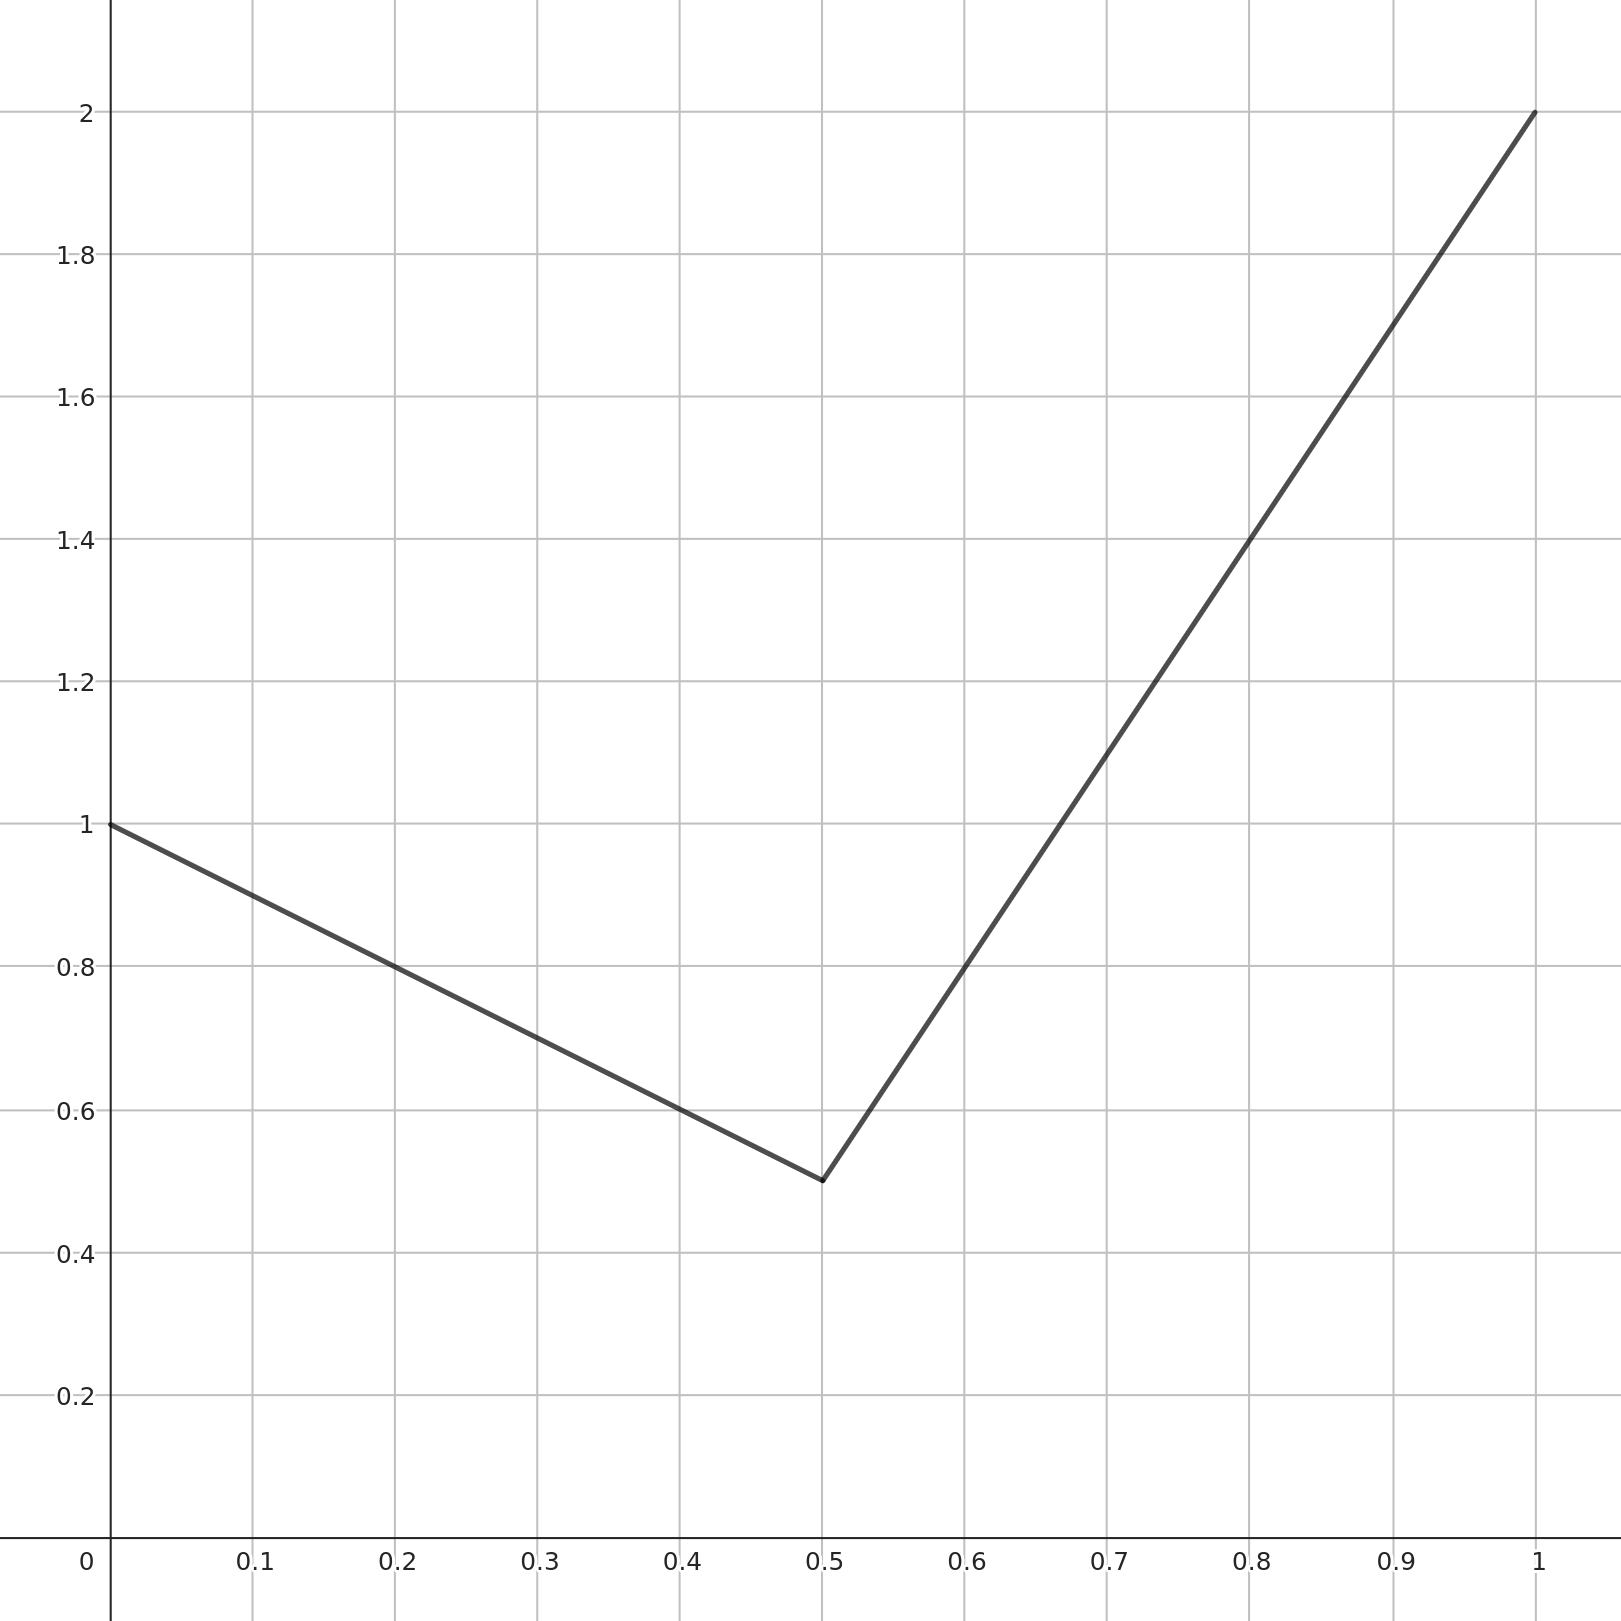
\includegraphics[scale=0.12]{rayon_spectral.png}
    \caption{Courbe représentative de la fonction $\rho \longmapsto r_{\sigma}(I - \rho A)$ sur $[0, 1]$}
    \label{fig:enter-label}
\end{figure}\newline
On constate alors que $r_{\sigma}(I - \rho A) < 1$ si et seulement si $\rho \in ]0,\frac{2}{3}[$. Ainsi, la méthode converge si et seulement si $\rho \in ]0,\frac{2}{3}[$ et le $\rho$ optimal est $\frac{1}{2}$ ($\rho$ pour lequel $r_{\sigma}(I - \rho A)$ est minimal). On précisera la raison pour laquelle on dit que ce $\rho$ est optimal dans la section Numérique. On remarque donc que la convergence de cette méthode ne dépend que de $\rho$ et pas de $x_0$.
\paragraph{Numérique}
On rappelle que pour tout $k \in \mathbb{N}$, $e_{k+1} = (I - \rho A)e_k$. Donc
$$
||e_{k+1}||_2 \leqslant |||(I - \rho A)|||_2 ||e_k||_2
$$
Mais puisque $A$ est symétrique, $I - \rho A$ est aussi symétrique, en particulier normale, donc $|||(I - \rho A)|||_2 = r_{\sigma}(I - \rho A)$. D'où
$$
||e_{k+1}||_2 \leqslant r_{\sigma}(I - \rho A) ||e_k||_2
$$
La convergence est donc linéaire. Ceci nous amène à définir le taux de convergence numérique (avec $N$ fixé suffisamment grand)
$$
r_{num}(\rho) = \frac{||e_N||_2}{||e_{N-1}||_2}
$$
Remarquons que plus ce taux est faible, meilleure est la vitesse de convergence et que ce taux est majoré par $r_{\sigma}(I - \rho A)$.\newline
Voici une représentation graphique de ce taux pour $\rho$ allant de $0$ à $1$ par pas de $0,01$ et $N = 30$.
\begin{figure}[h]
    \centering
    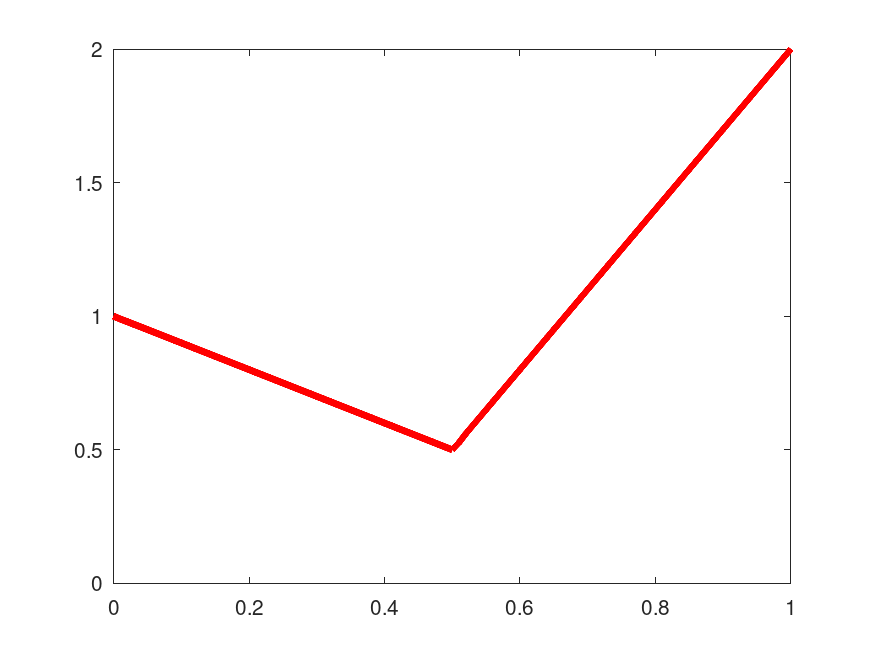
\includegraphics[scale=0.25]{TauxConvergence.png}
    \caption{Taux de convergence numérique pour $\rho$ allant de $0$ à $1$ par pas de $0,01$}
    \label{fig:enter-label}
\end{figure}\newline
On constate que cette représentation graphique coincide avec celle de $r_{\sigma}(I - \rho A)$. Donc la majoration du taux de convergence numérique par $r_{\sigma}(I - \rho A)$ est optimale et donc que l'algorithme converge le plus rapidement pour $\rho = \frac{1}{2}$ (d'où l'appellation du $\rho$ optimal).
\subsection{Méthode du gradient à pas optimal}
\subsubsection{Description de la méthode}
Soit $x_0 \in \mathbb{R}^n$. Dans le cas quadratique, on montre aisément que la méthode du gradient à pas optimal consiste à construire la suite $(x_k)_{k \in \mathbb{N}}$ de la manière suivante
$$
x_{k+1} = x_k - \rho_k \nabla J(x_k), \forall k \in \mathbb{N}
$$
avec $\rho_k =\dfrac{\lVert \nabla J(x_k)\lVert^2_2}{(A \nabla J(x_k),\nabla J(x_k))}$.\newline
\newline
On peut aussi montré que cette méthode converge pour toute donnée initiale $x_0$.
\subsubsection{Test de la méthode}
Pour tester cette méthode, on a pris $x_0 = 
\begin{pmatrix}
    0\\
    0
\end{pmatrix}$.\newline
On constate alors que l'algorithme converge en $55$ itérérations.\newline
Voici une représentation graphique de $f$ ainsi que la suite des itérés $(x_k,f(x_k))$.
\begin{figure}[h]
    \centering
    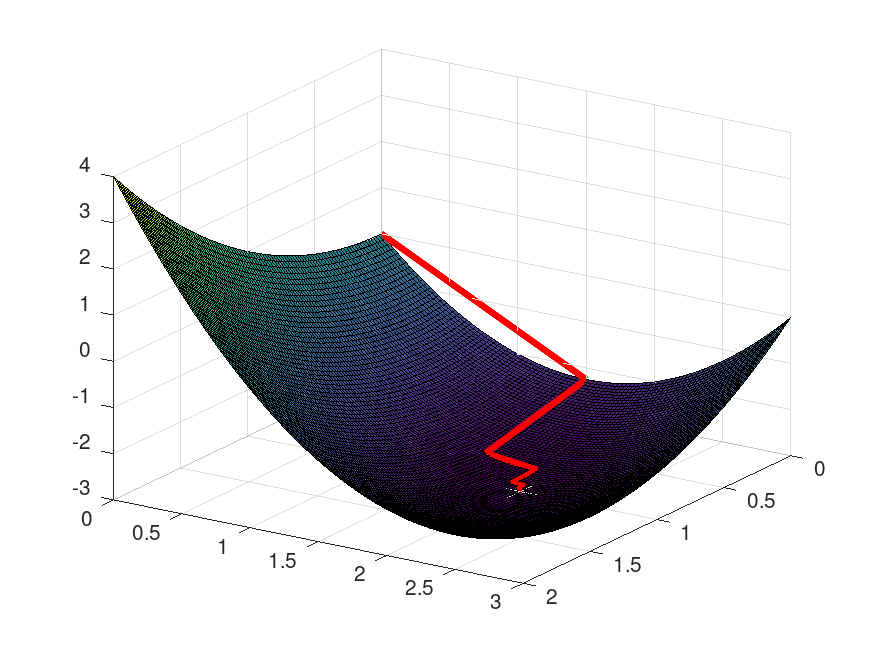
\includegraphics[scale=0.25]{GradientPasOptimal.png}
    \caption{Représentation graphique de $f$ et de la suite des itérés $(x_k,f(x_k))$}
    \label{fig:enter-label}
\end{figure}\newline
On observe bien que la suite "descend" vers le minimum de $f$ tout comme la méthode du gradient à pas constant mais de façon orthogonale (on a montré ce résultat en TD).
\subsection{Méthode du gradient conjugué}
\subsubsection{Description de la méthode}
Soit $x_0 \in \mathbb{R}^n$. Dans le cas quadratique, on a montré en TD que la méthode du gradient conjugué consiste à construire la suite $(x_k)_{k \in \llbracket 0,N_{\max} \rrbracket}$ (pour un certain $N_{\max} \in \llbracket 1,n \rrbracket $) de la manière suivante
$$
x_{k+1} = x_k + \rho_k d_k
$$
avec
$$
\left\{
\begin{array}{rl}
     g_0 &= A x_0 - b \\
     g_{k+1} &= g_k + \rho_k A d_k
\end{array}
\right.
$$
$$
\left\{
\begin{array}{rl}
    d_0 &= -g_0 \\
    d_{k+1} &= -g_{k+1} + \frac{(g_{k+1},g_{k+1})}{(g_k,g_k)}d_k
\end{array}
\right.
$$
$$
\left\{
\begin{array}{rl}
     \rho_0 &= -\frac{(g_0,d_0)}{(d_0,Ad_0)} \\
     \rho_{k+1} &= -\frac{(g_{k+1},d_{k+1})}{(d_{k+1},Ad_{k+1})}
\end{array}
\right.
$$
Ainsi construit, $x_{N_{\max}}$ est le point de minimum de $f$. La suite converge donc en un nombre fini d'itérations, ce qui est un avantage majeur.
\subsubsection{Test de la méthode}
Pour tester cette méthode, on a pris $x_0 = 
\begin{pmatrix}
    0\\
    0
\end{pmatrix}$.\newline
L'algorithme converge ici en $2$ itérations.\newline
Voici une représentation graphique de $f$ ainsi que la suite des itérés $(x_k,f(x_k))$.
\begin{figure}[h]
    \centering
    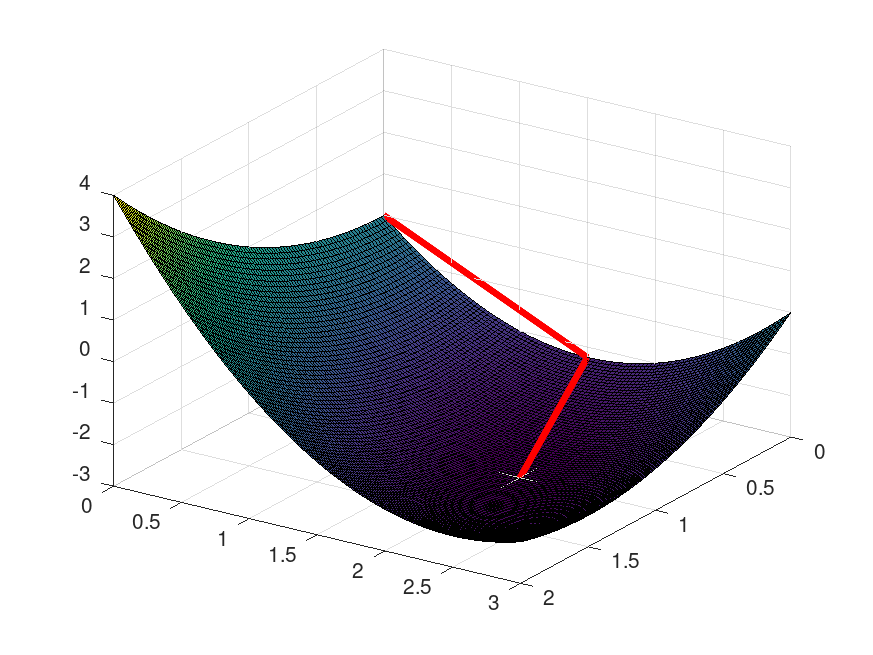
\includegraphics[scale=0.25]{GradientConjugue.png}
    \caption{Représentation graphique de $f$ et de la suite des itérés $(x_k,f(x_k))$}
    \label{fig:enter-label}
\end{figure}\newline
\subsection{Comparaison des méthodes}
Maintenant qu'on a implémenté et testé ces 3 algorithmes, on souhaite les classer pour savoir qui est "meilleur" que qui (en prenant $\rho = \frac{1}{2}$ pour la méthode du gradient à pas constant). Nous chercherons ici un moyen statistique pour classer ces algorithmes.
\subsubsection{Idée pour comparer}
Pour ce faire, on prendra $N$ valeurs de $x_0$ choisis aléatoirement (avec $N$ grand), on testera ces algorithmes pour chacun des $x_0$ et on stockera :
\begin{itemize}[label=\textbullet]
    \item le nombre d'itérations dans une matrice $nbIter$ de 3 lignes (correspondant aux 3 algorithmes) et de $N$ colonnes (correspondant aux $N$ valeurs de $x_0$)
\end{itemize}
On dira qu'un algorithme $A_1$ est meilleur qu'un algorithme $A_2$ au sens du nombre d'itérations si la moyenne du nombre d'itérations de $A_1$ est supérieur à $A_2$.
\subsubsection{Conclusion}
Grâce à ces deux relations transitives, on peut maintenant classer les algorithmes.\newline
En prenant $N = 1000$, on a trouvé que la méthode du gradient conjugué est melleure que la méthode du gradient à pas optimal qui est meilleure que la méthode du gradient à pas constant, et ce au sens du nombre d'itérations.\newline

Ainsi, de façon plutôt objective, on peut dire que la meilleure méthode est celle du gradient conjugué, ensuite il s'agit de celle du gradient à pas optimal, et enfin celle du gradient à pas constant.\newpage

D'une manière plus visuelle, voici une représentation graphique de l'erreur en fonction du nombre d'itérations pour chacun des algorithmes (pour $x_0 =
\begin{pmatrix}
    3\\
    1
\end{pmatrix}$).
\begin{figure}[h]
    \centering
    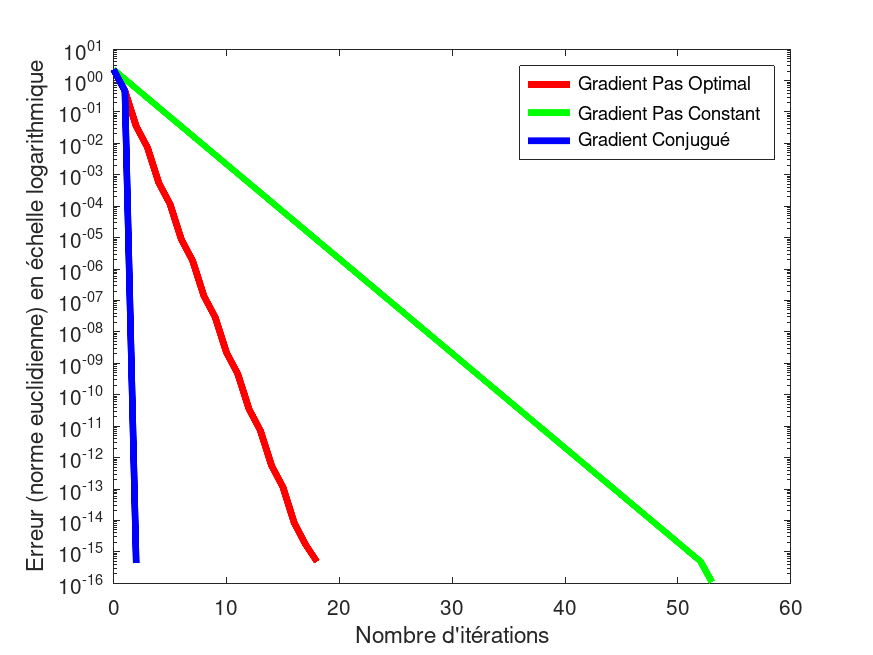
\includegraphics[scale=0.25]{Comparaison.png}
    \caption{Erreur (norme euclidienne) en fonction du nombre d'itérations pour $x_0 =
\begin{pmatrix}
    3\\
    1
\end{pmatrix}$}
    \label{fig:enter-label}
\end{figure}\newline
On aboutit à la même conclusion (et même mieux, l'erreur pour la méthode du gradient conjugué est toujours inférieure à celle pour la méthode du gradient à pas optimal qui est toujours inférieure à celle pour la méthode du gradient à pas constant, et ce pour n'importe quelle itération).
\subsubsection{Axes d'amélioration}
Un problème se pose. On a mené une comparaison des algorithmes pour une matrice $A$ et un vecteur $b$ prédéfini. On peut alors se demander si le classement dépend de ces derniers. Si ça se trouve, pour certaines matrices $A$ de très grande dimension, il est plus judicieux d'utiliser la méthode du gradient à pas optimal ou celle à pas constant plutôt que celle conjugué. Ce serait intéressant d'étudier ceci.\newline
On élimine la méthode du gradient à pas constant. En effet, les pas pour lesquels il y a convergence dépendent de la matrice $A$, ce qui est embêtant en pratique (il faudrait déterminer les pas qui permettent d'avoir la convergence, ce qui est assez fastidieux). Il nous reste les deux autres méthodes.\newline
Prenons par exemple la matrice de discrétisation du Laplacien en une dimension, qui est très utile en pratique, on l'utilise notamment lors de la résolution numérique d'EDP par des schémas aux différences finis (on peut montrer qu'elle est symétrique définie positive).\newline
On remarque que, pour $n = 100$, pour $x_0 = (0,...,0) \in \mathbb{R}^n$, et pour $x^* = (1,...,1) \in \mathbb{R}^n$ par exemple, on a :
\begin{itemize}[label=\textbullet]
    \item l'erreur initiale vaut $10$.
    \item l'erreur à la $20000^e$ itération vaut environ $0,000563648$ pour la méthode du gradient à pas optimal.
    \item l'erreur à la $51^e$ itération vaut environ $1,11 \times10^{-14}$ pour la méthode du gradient conjugué.
\end{itemize}
On observe alors que la méthode du gradient à pas optimal prend "beaucoup de temps" à converger (j'ai essayé pour un nombre plus élevé d'itérations pour la méthode du gradient à pas optimal mais mon ordinateur n'a pas apprécié...), ce qui pose problème (on a pris $n = 100$ seulement).\newline
On pourrait faire ce test pour différentes valeurs de $n$, de $x_0$, et de $x^*$ et arriver au même problème pour la méthode du gradient à pas optimal.\newline
Ainsi, il est bien plus commode d'utiliser la méthode du gradient conjugué.
% Gradient conjugué > Gradient pas Optimal > Gradient pas constant (pas optimal = 0.5)
% On pourrait tester aussi le temps de calcul
\section{Ouverture vers un autre problème}
Une des applications de l'optimisation est \textbf{l'apprentissage}. On est souvent amené en apprentissage à trouver les "meilleurs" paramètres, c'est-à-dire ceux qui minimisent une certaine fonction. C'est le cas du problème (2) et le problème alternatif (3), décris sur la feuille \textbf{optimisation : algorithme Adaboost et optimisation}.\newline
Pour résoudre le problème (3) (on peut facilement montrer que ce problème admet une unique solution), nous implémentons la méthode de relaxation et une variante (qu'on appellera relaxation modifiée). Nous remarquons alors que l'algorithme de relaxation modifiée nécessite au moins deux fois plus d'itérations que celui de relaxation non modifiée pour converger. Ce n'est pas très étonnant, c'est l'algorithme de relaxation non modifiée qu'on a étudié en cours.\newline

\end{document}